\documentclass[11pt]{article}
\usepackage[utf8]{inputenc}
\usepackage[T1]{fontenc}
\usepackage[francais]{babel}
\usepackage[francais]{layout}
\usepackage{hyperref}
\selectlanguage{french}

% NE PAS CHANGER !!
\ifx \public \undefined \def\public{etudiants} \fi
\usepackage[\public]{tps}
\usepackage{tikz}

% Numéro du TP
\newcommand{\numtd}{03}
% Titre du TP
\newcommand{\titretd}{Arithmetic logic unit and Register File}
\def\tup#1{\langle #1\rangle}
\begin{document}
	
	\entete{\numtd}{\titretd}


\section*{ALU}
We are going to design an eight-bit ALU that we will use it in the final phase of the project. The inputs of of this ALU are as the following:
\begin{itemize}
    \item Two 8-bit inputs as the operands.
    \item One 4-bit input to select the operation. 
    \item One 3-bit input to determine the numbers of bits that we use it for the \textbf{SHIFT} and \textbf{ROTATE}. 
\end{itemize}

And for the outputs, we have one 8-bit output for the result, a zero flag, a sign flag, and a carry flag. 

\begin{center}
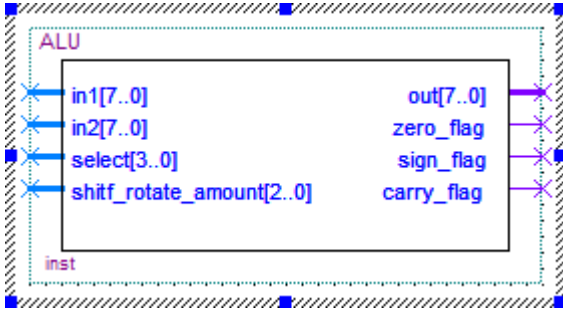
\includegraphics[width=10cm, height=5cm]{ALU.png}
\end{center}

The zero flag (rep. sign flag) will be set once the the result of ALU is zero (resp. negative).  And we set carry flag if one of the following occurs: 
\begin{itemize}
    \item There is a carry resulting from an addition operation.
    \item There is a borrow resulting from a subtraction operation.
    \item The overflow bit resulting from a binary shift operation or a rotate operation is 1.
\end{itemize}

\bigskip 


Once you are done with the design of the ALU, try some functional simulation. 

**Note that you can only use the primitives of Quartus. 

\bigskip

Bit shift examples for an eight-bit ALU:

\begin{center}
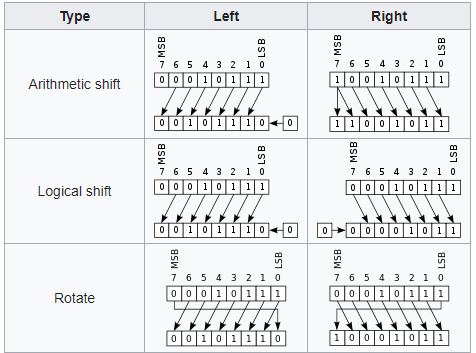
\includegraphics[width=10cm, height=5cm]{shift.png}
\end{center}

\bigskip

Here you can see the ALU Instructions:

\begin{center}
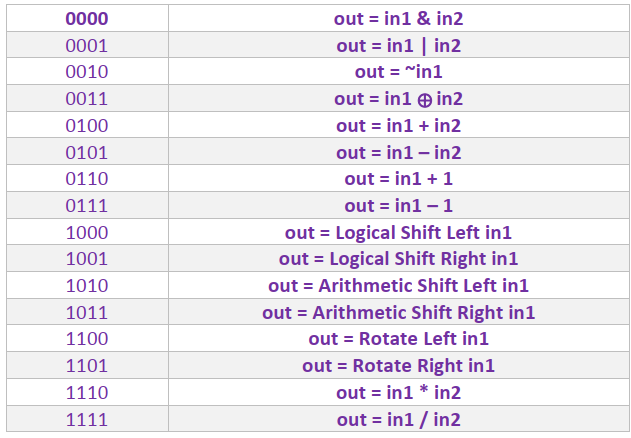
\includegraphics[]{Instructions.png}    
\end{center}


\section*{Register File}
A register is a set of flip-flops which each flip-flop capable of storing one bit of information. So, an n-bit register has a group of n flip-flops. In addition to flip-flops, a register may have logical gates that perform certain data-processing tasks. The flip-flops hold the binary information and the gates control when and how new information is transferred into the register. 

\bigskip

\subsubsection*{Question 1}
Using D Flip-Flops, construct an 8-bit register with a parallel load and also a clock input. That is to say this register has eight data input bits $D_0,\cdot,D_7$ and eight data output bits $O_0,\cdots,O_7$. In addition the register has a \textbf{Load} input which, when at logic level 1, sets the flip-flops data inputs to the register's eight input bits. When Load is at logic level 0, the eight flip-flops have their outputs fed into their inputs. This effectively disables loading from the four input bits.



\bigskip

Reminder: A simulation of D flip-flop with the clock input:

\begin{center}
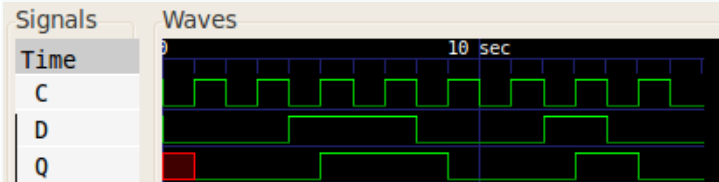
\includegraphics[width=8cm, height=2.5cm]{D.png}
\end{center}





\subsubsection*{Question 2}
A register file is an array of registers. Design an eight-bit register file that has four registers. The block diagram of it is as follows: 

\begin{center}
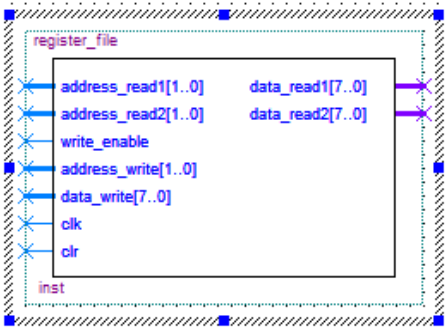
\includegraphics[width=10cm, height=5cm]{register file.png}    
\end{center}

Description of the register file: 

\begin{itemize}
    \item The output of two registers, which are determined by \textbf{address-read1} and \textbf{address-read1}, will be sent to \textbf{data-read1} and \textbf{data-read2} respectively.
    \item If \textbf{write-enable} is 1 and the edge of the clock is rising, then the \textbf{data-write} will be sent to the register with the address "\textbf{address-write}".
    \item If \textbf{clr} is 1, then the output of all registers will be zero. 
\end{itemize}


\end{document}
